\section*{Chapter 1: Introduction}
\setcounter{section}{1} \setcounter{subsection}{0}
\addcontentsline{toc}{section}{\textit{Chapter 1: Introduction}}

The \textit{Introduction} is one of the most important parts of your report as it gives a brief overview that will make the reader understand (i) what you set out to do and (ii) what you achieved. Many readers will read the \textit{Introduction} first and then the  \textit{Conclusions} to get an overview before reading the detail – so it is important that both sections are very carefully written.

It is very important that \textit{Introduction} introduces the \textbf{report} and the \textbf{project} – it is not there to introduce the subject in general.

There are no rules on how to write an introduction, but it should include what the project is about, give \textit{a very short description} of the technical context in which the project is carried out and explain the motivation for the work. If you are doing an implementation project it must explain what functionality the system \textbf{realises}, and if you are doing a research project what is the novelty of the approach used. 

Very importantly, it should clearly indicate what you have done for the project. 

A good introduction should be no more than 4 pages.
\subsection{Format}
\subsubsection{Format for headings}
Format for level 1, 2 and 3 headings is given in this template; just choose the relevant style from the format list.

\subsubsection{Format for body text}
Font Times New Roman, Font size should be 12pt, 1.5 line spacing in and justified. Do not indent the first line.
% the default setting in LaTeX already satisfies the above theme.

\subsubsection{Format for equations}
Equations should be centred with a numbered caption on the right; an example is below:
\begin{equation}
I_{\,i, own}=P_{\,total, j} \cdot \gamma_{\,i, j} - P_{\,i,recv}
\end{equation}

\subsubsection{Format for figures}

Figures should be centred and followed by captions. Captions should be centred, 10pt font 
Times New Roman Bold. Use automatic numbering without chapter number for captions. Select “Caption” from Styles and Formatting to format captions.

Whenever you include a figure in your document you must reference it in the text e.g. this is a reference to Figure\ref{fig:examplefig}.

When presenting graphs, make sure you label the axes and include units where applicable. Also include a legend (i.e. key) where appropriate.

\begin{figure}[h]
\centering
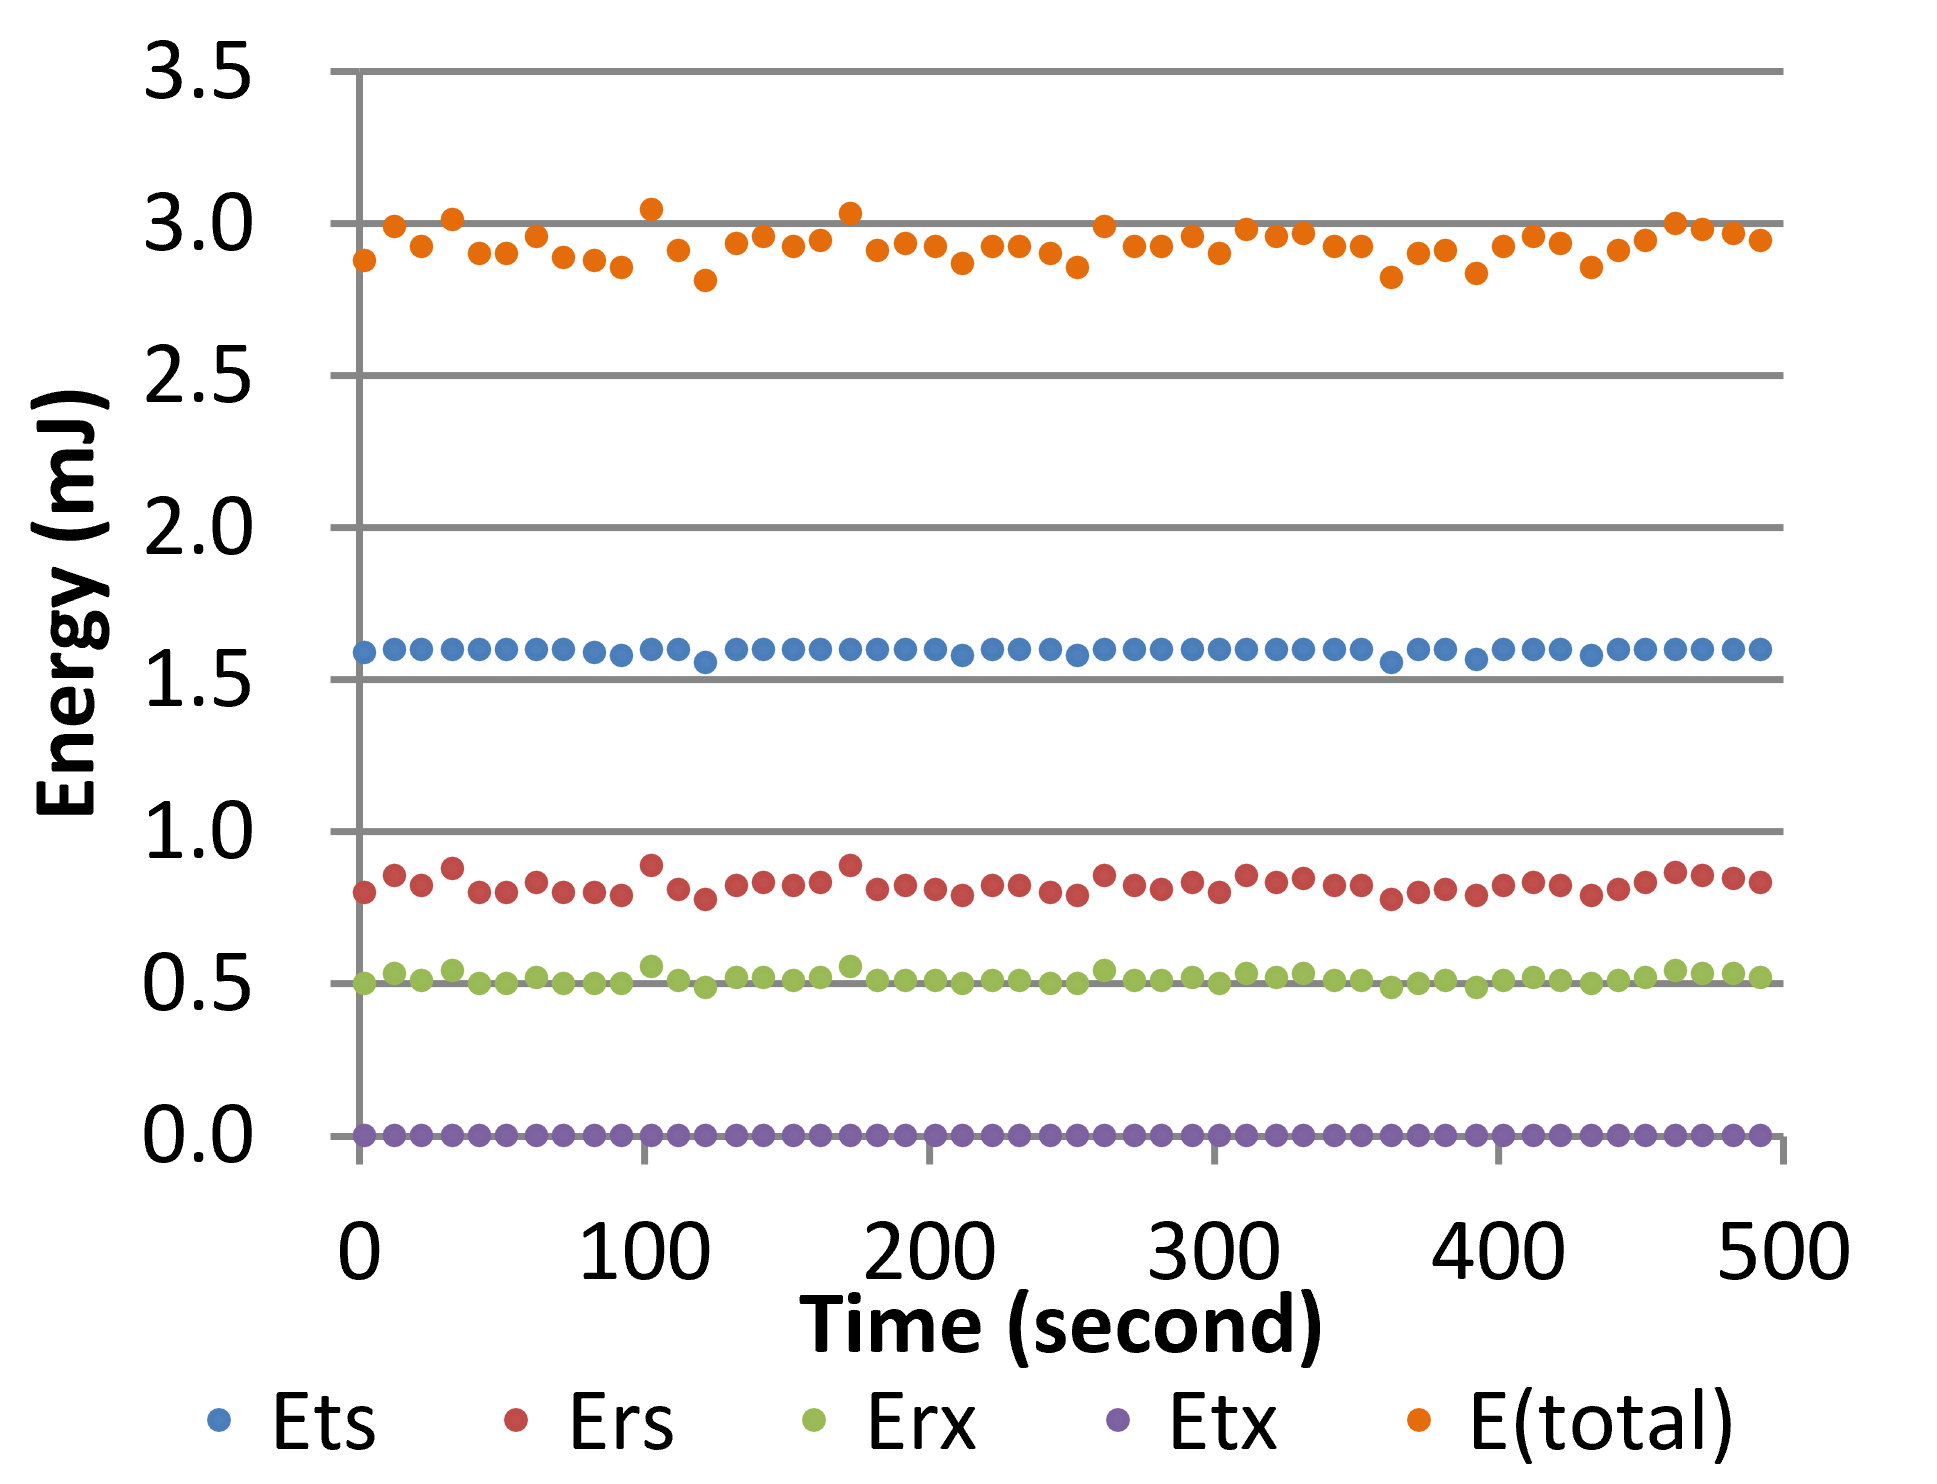
\includegraphics[width=10cm]{figures/examplefig.PNG}
\caption{Comparison of energy components}
\label{fig:examplefig}
\end{figure}

\subsubsection{Format for Tables}
Unlike figures, the caption for a table should be before the table; Table\ref{table:exampletable} shows an example of the correct layout.


\begin{table}[h]  
  \centering  
  \begin{spacing}{1.35}  
  \caption{Example Table}\vspace{0.7em}
  \label{table:exampletable} 
    \begin{tabular}{|p{4cm}|p{4cm}|p{4cm}|}   
    \hline
     & & \\  
    \hline
     & & \\
    \hline
     & & \\
    \hline
    \end{tabular}
  \end{spacing}
\end{table}
